% ================================================================
% LaTeX Template, contains guidelines on coding practice and includes extended 
%   functionality on top of the beamer class, to be used for presentations.
% 
% Created from accumulated spaghetti code from my masters presentations from 
%   2015--2018 and various excerpts from StackExchange and Github, motivated by 
%   a literature review presentation.
%
% Written by Blake Cook on 2019-02-22.
% Copyright (c) 2019. All rights reserved.
% 
% ================================================================
% SET DOCUMENT FIELDS

% Required fields
\def\DOCTITLE{Document Title}
\def\AUTHOR{Author}

% Optional fields (comment out fields that are not needed)
\def\PROJECTTITLE{Project Title}
\def\PROJECTSUBTITLE{Project Subtitle}
\def\DEPARTMENT{Department}
\def\INSTITUTION{Institution}
\def\TIMEZONE{GMT}


% ================================================================
% SET DOCUMENT PARAMETERS

% Main
\documentclass[
  11pt,            % Default font size
  aspectratio=43   % Aspect ratio
]{beamer}

% [USER] Review mode
%   Toggles timestamp on titlepage and notes appearance
\def\draft{1}  


% ================================================================
% LOAD PREAMBLE
% ================================================================
% LOAD PACKAGES THAT ONLY NEED DEFAULT OPTIONS

% Default AMS packages
\usepackage{
  amsmath,   % Extended equation environments
  amssymb,   % Extended maths symbols (also loads amsfonts)
  amsthm,    % Theorem-like structures
} 

% Graphics packages
\usepackage{
  caption,     % Write captions 
  graphicx,    % Include graphics (with extras)
  pgfplots,    % For charts
  tikz,        % Draw tikz pictures
  subcaption,  % Write subcaptions
}
\pgfplotsset{compat=1.13}  % set version

% Formatting packages
\usepackage{
  datetime,    % Output date and time 
  fancyhdr,    % Extended header and footer options 
  hyperref,    % Generate hyperlinks for references
  multicol,    % Multicolumn environment
  natbib,      % Better inline citations (\citep, \citet, \citeauthor)
}


% ================================================================
% LOAD PACKAGES THAT NEED CONFIG OPTIONS AND USER PACKAGES

% required for \source command
\usepackage[
  absolute,
  overlay
]{textpos}  


% ================================================================
% DECLARE MATHS MACROS 

% Common symbols
\def\vep{\varepsilon}           % \vep - Script eps
\def\del{\partial}              % \del Partial derivative
\def\P{\mathbb{P}}              % \P - Probability measure
\def\E{\mathbb{E}}              % \E - Expectation operator
\def\Var{\text{Var}}            % \Var - Variance operator
\def\Cov{\text{Cov}}            % \Cov - Covariance
\def\F{\mathcal{F}}             % \F - Sigma-field
\def\Tr{\text{Tr}}              % \Tr - Matrix trace
\def\Det{\text{Det}}            % \Det - Matrix determinant
\def\grad{\boldsymbol{\nabla}}  % \grad - Gradient operator
\def\lap{\nabla^2}              % \lap - Laplacian
\def\I{\mathbb{I}}              % \I - Indicator 

% Common structures
\newcommand{\br}[1]{\left \lbrace #1 \right \rbrace}     % \br{.} - braces
\newcommand{\abs}[1]{\left \vert #1 \right \vert}        % \abs{.} - abs val
\newcommand{\floor}[1]{\left \lfloor #1 \right \rfloor}  % \floor{.} - floor
\newcommand{\ceil}[1]{\left \lceil #1 \right \rceil}     % \ceil{.} - ceiling 
\newcommand{\norm}[1]{\left \|#1 \right \|}              % \norm{.} - norm
\newcommand{\vc}[1]{\boldsymbol{#1}}                     % \vc{.} - vector (bb)

\newcommand{\ncr}[2]{  % \ncr{}{} - Combination
  \left(               % e.g. \ncr{25}{3}
    \begin{matrix} 
      #1 \\ #2 
    \end{matrix} 
  \right)
}

\newcommand{\ddx}[3][]{  % \ddx[]{}{} - Derivative operator 
  \frac{d^{#1} {#2}}     % e.g. \ddx{f}{x}, \ddx[2]{f}{x}
    {d{#3}^{#1}}  
} 

\newcommand{\ppx}[3][]{      % \ppx[]{}{} - Partial derivative operator 
  \frac{\partial^{#1} {#2}}  % \ppx{f}{x}, \ppx[2]{f}{x}
    {\partial{#3}^{#1}}      % TODO: update command for mixed partials
}


% ================================================================
% DOCUMENT FORMATTING

% Define \source{} to place references in bottom left of slides
\newcommand\source[1]{
  \begin{textblock*}{0.66\paperwidth}[0,1](6pt,1.055\textheight)
    \usebeamerfont{framesource}
    \usebeamercolor[fg]{framesource} 
    \fontsize{6pt}{7.2}
    \selectfont 
    \raggedright 
    Source: #1
    \hspace{.5em}
  \end{textblock*}
}

% Define commands to switch navigation bullets on and off
% Source: https://tex.stackexchange.com/a/45038
\makeatletter
  \let\beamer@writeslidentry@navbulon
    =\beamer@writeslidentry

  \def\beamer@writeslidentry@navbuloff{
    \expandafter\beamer@ifempty\expandafter{
      \beamer@framestartpage
    }{}% does not happen normally
    {%else
      % removed \addtocontents commands
      \clearpage
      \beamer@notesactions
    }
  }

  \newcommand*{\navbulon}{
    \let\beamer@writeslidentry=
      \beamer@writeslidentry@navbulon
  }

  \newcommand*{\navbuloff}{
    \let\beamer@writeslidentry=
      \beamer@writeslidentry@navbuloff
  }
\makeatother

% Define \outline environment, only appears if \draft=1
\newenvironment{outline}{
  \if\draft1
    \navbuloff
    \begin{frame}[plain]
}{
    \end{frame}
    \navbulon
  \fi
}


% Select beamer theme
\usetheme{Frankfurt}

% Select beamer colours
\definecolor{UOMblue}{RGB}{0,69,124}
\usecolortheme[named=UOMblue]{structure}

% Define date format for final
\newdateformat{monthyeardate}{
  \monthname[\THEMONTH], \THEYEAR
}

% Define date format for draft
\newdateformat{draftdate}{
  DRAFT \\
  \currenttime 
  \ifx\TIMEZONE\undefined
  \else
    \space \TIMEZONE 
  \fi
  \space - \space 
  \ordinal{DAY} of \monthname[\THEMONTH], 
  \THEYEAR
}

% Write outline of section slide on each new section
\AtBeginSection[]
{
  \navbuloff
	\begin{frame}<beamer>{Outline}
		\tableofcontents[currentsection,hideothersubsections]
  \end{frame}
  \navbulon
}

% Clear section title for references
\renewcommand\bibsection{}




% ================================================================
% WRITE DOCUMENT
\begin{document}

  % PRINT TITLEPAGE
  \ifx\PROJECTTITLE\undefined
  % If PROJECTTITLE is not given, 
  % print DOCTITLE as focus (REQUIRED)
  \title{\DOCTITLE}
\else
  % If PROJECTTITLE is given,
  % print DOCTITLE (REQUIRED) 
  % underneath PROJECTTITLE (and PROJECTSUBTITLE)
  \ifx\PROJECTSUBTITLE\undefined
    % If PROJECTSUBTITLE is not given, 
    % print PROJECTTITLE as focus
    \title{\PROJECTTITLE}
    \else
    % If PROJECTSUBTITLE is given,
    %  print PROJECTTITLE and PROJECTSUBTITLE as focus
    \title{
      \PROJECTTITLE \\
      \PROJECTSUBTITLE
    } 
  \fi
  % print DOCTITLE (REQUIRED) underneath PROJECTTITLE
  \subtitle{\DOCTITLE}
\fi


\author{\AUTHOR}

\institute{
  \DEPARTMENT \\ 
  \INSTITUTION
}

\if\draft1
  \draftdate
\else
  \monthyeardate
\fi

\date{\today}


% Print titlepage
\begin{frame}
	\titlepage
\end{frame}

% Print contents slide (list sections)
\begin{frame}{Outline}
	\tableofcontents[hideothersubsections]
\end{frame}


  % PRINT NOTES IN PREFACE IF DRAFTING
  \if\draft1
  
    % Enable roman page numbering for review notes
    \pagenumbering{roman}  

    \begin{frame}{DRAFT: NOTES}

  \begin{itemize}
      \item Write sections
  \end{itemize}
  
\end{frame}


    
    % Enable arabic page numbering for document
    \pagenumbering{arabic}  
    
  \fi


  % WRITE MAIN DOCUMENT MATTER

  \section{A section}

\begin{frame}{\insertsectionhead}
  
  ``Movement of a motile cell or organism, 
  or part of one, 
  in a direction corresponding to 
  a gradient of increasing or decreasing concentration 
  of a particular substance.''
  
  \vspace*{9pt}
  
  \begin{itemize}
    \item Directed movement of cells tends to be in response to 
    signalling molecules, 
    released by other cells in minuscule amounts
    \begin{itemize}
      \item E.g. 
      Development of tissue and organs, 
      Immune system cell response to pathogens
    \end{itemize}
  \end{itemize}
  
  \vspace*{9pt}
  
	\underline{Do cells respond in a similar way to electrical fields?}
  
\end{frame}


\subsection{Subsection}

\begin{frame}{\insertsubsectionhead}
  
  E.g. E. Coli 'run and tumble' motion

	\begin{figure}[h!]
    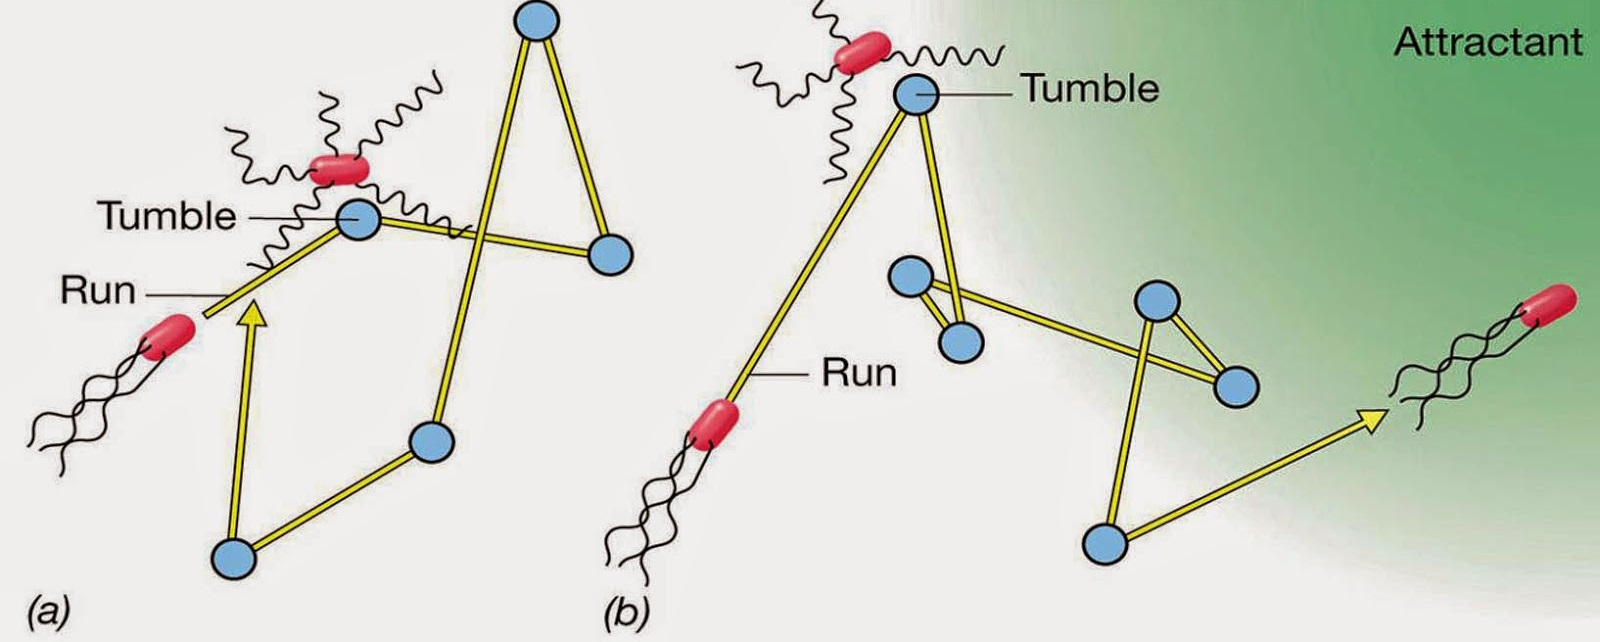
\includegraphics[width=0.7\textwidth]{src/img/example0}
		\caption{E. Coli chemotaxis}
		\source{\url{http://biologicalexceptions.blogspot.co.uk/2014/09/}}
  \end{figure}
  
	\begin{itemize}
    \item Cell swims in a direction and 
      randomly change direction after 
			'tumbling' at random times
		\begin{itemize}
      \item Direction chosen is biased towards 
        positive nutrient gradients
		\end{itemize}
	\end{itemize}

\end{frame}


\subsection{Another subsection}

\begin{frame}{\insertsubsectionhead}

  But not all motile cells have flagella..
  
  \begin{figure}
    
		\begin{subfigure}{0.4\textwidth}
			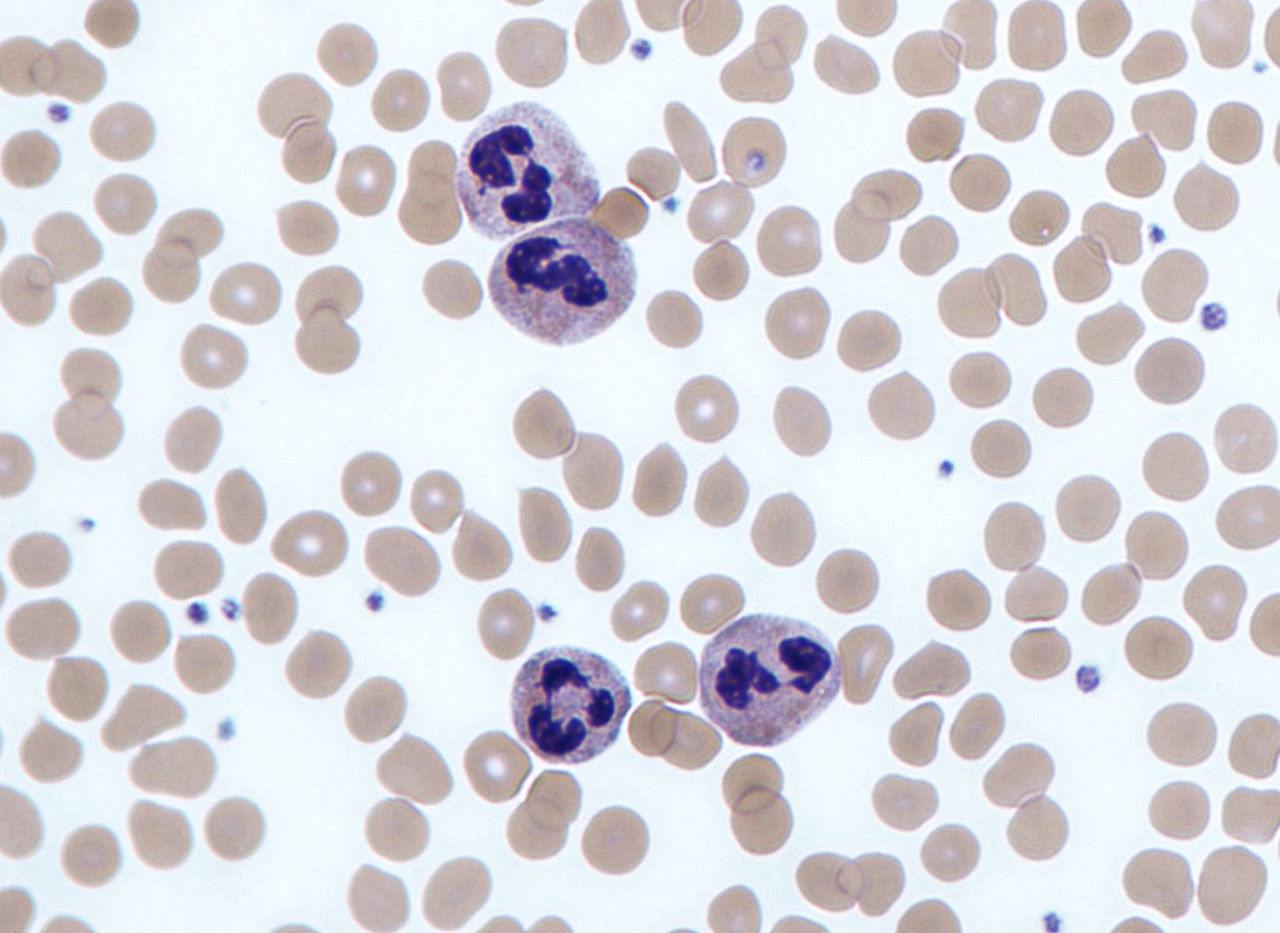
\includegraphics[width=\textwidth]{src/img/example1}
			\caption{White blood cells}
		\end{subfigure}
		\begin{subfigure}{0.44\textwidth}
			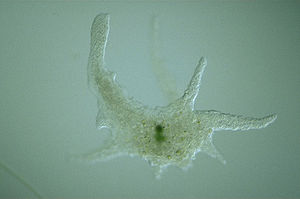
\includegraphics[width=\textwidth]{src/img/example2}
			\caption{Amoeba}
		\end{subfigure}
    
    \source{
      Wikipedia entries, 
        \textit{Neutrophil}, 
        and \textit{Chaos (genus)},  \\
      \url{https://en.wikipedia.org/wiki/File:Neutrophils.jpg}  \\
      \url{https://en.wikipedia.org/wiki/File:Chaos_carolinense.jpg}
    }
	\end{figure}

\end{frame}

\begin{frame}{Differently named frame}

  But not all motile cells have flagella..
  
  \begin{figure}
    
		\begin{subfigure}{0.4\textwidth}
			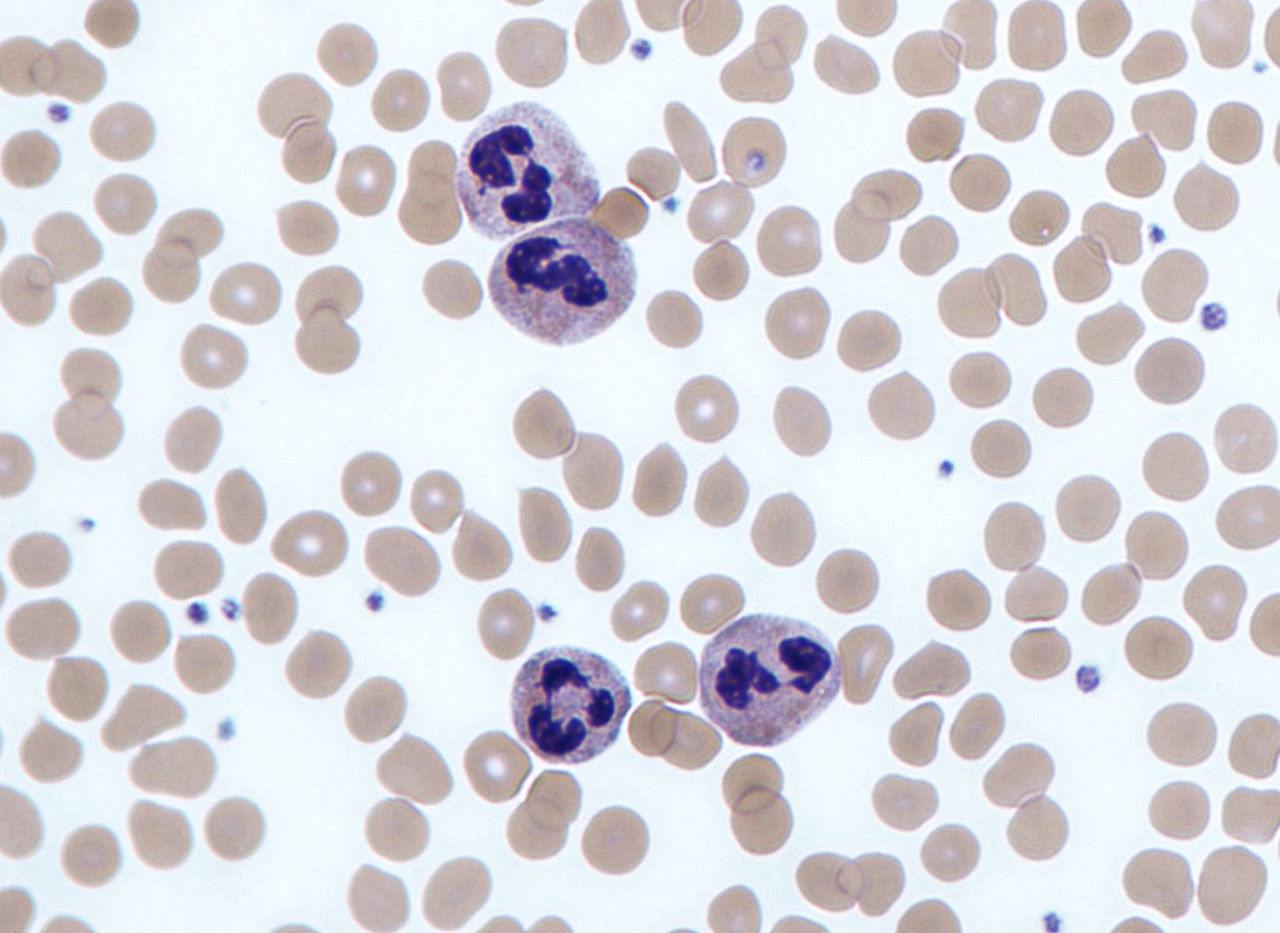
\includegraphics[width=\textwidth]{src/img/example1}
			\caption{White blood cells}
		\end{subfigure}
		\begin{subfigure}{0.44\textwidth}
			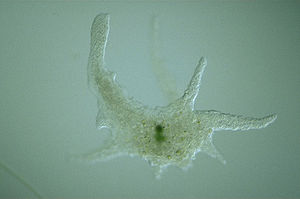
\includegraphics[width=\textwidth]{src/img/example2}
			\caption{Amoeba}
		\end{subfigure}
    
    \source{
      Wikipedia entries, 
        \textit{Neutrophil}, 
        and \textit{Chaos (genus)}, 
      \url{https://en.wikipedia.org/wiki/File:Neutrophils.jpg}  
      \url{https://en.wikipedia.org/wiki/File:Chaos_carolinense.jpg}
    }
	\end{figure}

\end{frame}

  \section{Another section}

\subsection{Yet another subsection}

\begin{frame}{\insertsubsectionhead}

  Let \( \br{\vc{r}_1, ..., \vc{r}_n} \) be 
    positions of nodes on cell surface and 
    let \( \mathcal{N}_i(t) \) denote 
    the neighbouring nodes of 
    node \( i \) at time \( t \). 

	\vspace*{12pt}
  
  Assume inertial terms are small enough to be 
    inconsequential compared to
    dissipative terms 
    in equation of motion:

	\begin{align*}
		\eta \ddx{\vc{r}_i}{t} = \vc{B}_i(t)\; + 
			\sum_{j\in \mathcal{N}_{i}(t)} \vc{F}_{i j}(t),
  \end{align*}
  
  where \( \eta \) is a drag coefficient, 
    \(\vc{F}_{i j}\) denotes the force on node \(i\) from node \(j\) and 
    \(\vc{B}_i(t)\) is the sum of other forces on node \(i\) at time \(t\).	

\end{frame}


  % WRITE FORMATTED REFERENCES AND END OF PRESENTATION

  
\navbuloff

\begin{frame}{References}
  
  \fontsize{6pt}{7.2}
  \selectfont
  
  \nocite{Buzsaki2012}
  \nocite{niedermeyer1972generalized}
  
  \bibliographystyle{humannat}
	\bibliography{\jobname-refs} 
  
  \vspace{24pt}
  
  \fontsize{12pt}{7.2}
  \selectfont
  
  Thank you for your time!
  
\end{frame}


% Insert black slide as final
\appendix
\bgroup

  \setbeamercolor{background canvas}{bg=black}
  \setbeamertemplate{navigation symbols}{}

  \begin{frame}[plain]{}
  \end{frame}

\egroup


\navbulon

  % WRITE BACKUP SLIDES

  \appendix

\navbuloff

\begin{frame}{Backup slide}
  Backup stuff
\end{frame}

\navbulon




\end{document}
